\documentclass[conference]{IEEEtran}
\IEEEoverridecommandlockouts
\usepackage{cite}
\usepackage{amsmath,amssymb,amsfonts}
\usepackage{algorithmic}
\usepackage{graphicx}
\usepackage{textcomp}
\usepackage{xcolor}
\usepackage{booktabs}
\usepackage{multirow}
\usepackage{array}

\def\BibTeX{{\rm B\kern-.05em{\sc i\kern-.025em b}\kern-.08em
    T\kern-.1667em\lower.7ex\hbox{E}\kern-.125emX}}

\begin{document}

\title{Physics-Informed Dynamic Thresholding and TinyML Quantization for Low-Latency 5G O-RAN Handover Optimization\\
}

\author{\IEEEauthorblockN{Himanshu Kumar}
\IEEEauthorblockA{\textit{Department of Electronics and Communication Engineering} \\
\textit{Indian Institute of Technology / Autonomous Systems Laboratory}\\
India \\
himanshu-2l@users.noreply.github.com}
}

\maketitle

\begin{abstract}
Open Radio Access Network (O-RAN) architectures introduce Near-Real-Time RAN Intelligent Controllers (Near-RT RIC) operating within $10$--$1000$~ms control loops to optimize mobility management via xApps. However, conventional 3GPP A3 event-triggered handover algorithms rely on static Reference Signal Received Power (RSRP) thresholds and fixed Time-to-Trigger (TTT) windows, failing to adapt to rapid fading dynamics and causing unnecessary Ping-Pong handovers or Radio Link Failures (RLFs). Moreover, deploying complex machine learning models directly on resource-constrained edge RIC controllers introduces unacceptable RAM consumption and inference latency. To overcome these limitations, this paper proposes a novel 3-Pillar Framework: 1) a Kinematic Physics-Informed Feature Layer extracting $1^{\text{st}}$-order RSRP Velocity ($v = \frac{d\text{RSRP}}{dt}$) and $2^{\text{nd}}$-order RSRP Acceleration ($a = \frac{d^2\text{RSRP}}{dt^2}$) to provide temporal fading dynamics; 2) Cost-Sensitive Dynamic Adaptive Thresholding (DAT) minimizing operational cost $\mathcal{C}(P_{\text{th}}) = w_1 N_{\text{PingPong}} + w_2 N_{\text{RLF}}$ under asymmetric penalties ($w_2/w_1 = 5$); and 3) Edge TinyML Dynamic INT8 Quantization and Decision Tree Pruning for near-zero latency RIC execution. Evaluated under 10 runs of 5-fold Stratified Cross-Validation on both a real-world 5G drive-test dataset (ANATEL, $N=1,458$) and a 3GPP-compliant ns-3 simulation dataset ($N=3,922$), kinematic features (`energy\_accel` and `energy\_velocity`) rank \#1 in feature importance across all classifiers. DAT shifts optimal probability thresholds to $P_{\text{th}}^* = 0.35$ (real) and $0.46$ (simulated), reducing RLFs by 81.9\% and total operational costs by 44.7\%. Finally, INT8 quantization compresses model footprint by 56.8\% ($29.64$~KB to $12.80$~KB) with only 0.64\%--1.37\% accuracy loss, while pruned decision trees achieve $0.096$~ms latency—comfortably satisfying Near-RT RIC SLA constraints.
\end{abstract}

\begin{IEEEkeywords}
5G O-RAN, Near-RT RIC, Handover Optimization, Kinematic Feature Engineering, Dynamic Thresholding, TinyML, INT8 Quantization, Radio Link Failure.
\end{IEEEkeywords}

\section{Introduction}
The architectural transition toward Open Radio Access Networks (O-RAN) decoupled proprietary RAN hardware from software, introducing standardized service models (E2SM) and intelligent controllers (RIC) \cite{oran_arch}. Among these, the Near-Real-Time RIC (Near-RT RIC) operates on control loops between $10$~ms and $1000$~ms, enabling intelligent radio resource management (RRM) and mobility optimization via embedded software applications termed xApps \cite{oran_ric}.

Handover (HO) decision-making remains one of the most critical mobility functions in dense 5G New Radio (NR) networks. Standardized 3GPP A3 event-triggered algorithms evaluate whether neighbor cell signal strength exceeds serving cell signal strength by a fixed hysteresis margin ($H_y$) over a predefined Time-to-Trigger ($TTT$) interval \cite{3gpp_38300}:
\begin{equation}
\text{RSRP}_{\text{target}}(t) - \text{RSRP}_{\text{serving}}(t) > \text{A3}_{\text{offset}} + H_y
\end{equation}
While deterministic, this rule-based mechanism exhibits severe vulnerabilities under modern user equipment (UE) mobility. In urban propagation environments characterized by log-normal shadowing, multipath fading, and variable UE velocity, fixed A3 parameters lead to two failure modes:
\begin{enumerate}
    \item \textbf{Ping-Pong Handovers (False Positives):} Unnecessary back-and-forth handovers triggered by momentary signal spikes, degrading throughput and consuming core network signaling capacity.
    \item \textbf{Radio Link Failures (False Negatives):} Delayed handovers caused by sudden deep fading or rapid UE departure, resulting in connection drops, RRC re-establishment delays, and user Quality of Experience (QoE) degradation.
\end{enumerate}

Existing machine learning (ML) handover predictors often feed raw 50-sample RSRP sliding windows into heavy deep neural networks or ensemble classifiers \cite{paper1}. However, two fundamental gaps remain in literature:
\begin{enumerate}
    \item \textbf{Lack of Physical Kinematic Context:} Pure RSRP amplitude sequences lack explicit trajectory and fading velocity context, forcing models to infer signal drift rates implicitly.
    \item \textbf{RIC Edge Resource Constraints:} Deploying uncompressed Random Forest ensembles ($>3.7$~MB RAM) or unquantized neural networks on Near-RT RIC edge nodes violates strict L1/L2 memory limits and sub-10~ms control loop SLAs.
\end{enumerate}

To address these challenges, this paper presents a complete **3-Pillar Framework** for 5G O-RAN Handover Optimization:
\begin{itemize}
    \item \textbf{Pillar 1 (Kinematic Physics-Informed Feature Layer):} Derives $1^{\text{st}}$-order RSRP Velocity ($v_t$) and $2^{\text{nd}}$-order RSRP Acceleration ($a_t$) sequences, alongside window-level kinematic energy proxies (`energy\_accel`, `energy\_velocity`).
    \item \textbf{Pillar 2 (Cost-Sensitive Dynamic Adaptive Thresholding):} Formulates threshold selection as a cost-minimization function $\mathcal{C}(P_{\text{th}})$, penalizing catastrophic RLFs 5$\times$ more heavily than Ping-Pong events.
    \item \textbf{Pillar 3 (Edge TinyML Quantization \& Latency Profiling):} Applies PyTorch INT8 dynamic quantization and decision tree pruning, reducing memory footprint by 56.8\% while maintaining sub-millisecond execution time.
\end{itemize}

The remainder of this paper is organized as follows: Section~\ref{sec:system_model} details the system model and mathematical formulation. Section~\ref{sec:framework} details the 3-Pillar Framework. Section~\ref{sec:experiments} presents cross-validation results across real and simulated datasets. Section~\ref{sec:conclusion} concludes the paper.

\section{System Model \& Problem Formulation}
\label{sec:system_model}

\subsection{Temporal RSRP Signal Representation}
Consider a UE navigating through a heterogeneous 5G NR cellular layout. At discrete sampling interval $\Delta t$, the UE measures the RSRP of the serving gNodeB (gNB). Over a sliding temporal window of length $N = 50$, the raw signal measurement vector is defined as:
\begin{equation}
\mathbf{R} = [r_0, r_1, r_2, \dots, r_{N-1}]^T \in \mathbb{R}^{N}
\end{equation}
where $r_t$ represents the instantaneous RSRP measurement in dBm at time step $t$.

\subsection{Kinematic Derivative Formulation}
To incorporate physical mobility kinetics into the feature space without requiring external GPS instrumentation, we construct $1^{\text{st}}$-order and $2^{\text{nd}}$-order finite difference sequences across the time-series vector $\mathbf{R}$.

\subsubsection{RSRP Velocity Sequence ($\mathbf{V}$)}
The discrete $1^{\text{st}}$-order derivative represents the signal drift velocity $v_t$:
\begin{equation}
v_t = \frac{r_t - r_{t-1}}{\Delta t}, \quad t \in \{1, 2, \dots, N-1\}
\end{equation}
Assuming uniform time steps $\Delta t$, $v_t$ measures instantaneous attenuation rate in dBm/step. Positive velocity indicates UE motion toward the cell center, whereas negative velocity indicates UE departure toward the cell boundary.

\subsubsection{RSRP Acceleration Sequence ($\mathbf{A}$)}
The discrete $2^{\text{nd}}$-order derivative captures rate of change of signal velocity (acceleration) $a_t$:
\begin{equation}
a_t = \frac{v_t - v_{t-1}}{\Delta t} = r_t - 2r_{t-1} + r_{t-2}, \quad t \in \{2, 3, \dots, N-1\}
\end{equation}
RSRP acceleration isolates high-frequency multipath fading volatility and abrupt physical trajectory changes.

\subsubsection{Kinematic Energy Proxies}
We define window-aggregated RMS kinematic energy indicators:
\begin{equation}
E_v = \sqrt{\frac{1}{N-1}\sum_{t=1}^{N-1} v_t^2}, \quad E_a = \sqrt{\frac{1}{N-2}\sum_{t=2}^{N-1} a_t^2}
\end{equation}
where $E_v$ quantifies overall fading intensity, and $E_a$ serves as a kinematic jerk-energy proxy.

\subsection{Asymmetric Operational Cost Minimization}
Let $y_i \in \{0, 1\}$ represent the ground-truth handover label for sample $i$, where $y_i = 1$ indicates a necessary handover execution. Given a predicted probability $\hat{p}_i = P(y_i = 1 | \mathbf{X}_i)$ generated by an ML model, a decision rule applies threshold $P_{\text{th}}$:
\begin{equation}
\hat{y}_i(P_{\text{th}}) = 
\begin{cases} 
1, & \text{if } \hat{p}_i \ge P_{\text{th}} \\
0, & \text{if } \hat{p}_i < P_{\text{th}}
\end{cases}
\end{equation}

Classification errors map directly to operational network events:
\begin{itemize}
    \item \textbf{False Positives (FP):} $\hat{y}_i = 1, y_i = 0 \Rightarrow N_{\text{PingPong}}$ (Unnecessary Handover).
    \item \textbf{False Negatives (FN):} $\hat{y}_i = 0, y_i = 1 \Rightarrow N_{\text{RLF}}$ (Radio Link Failure).
\end{itemize}

Conventional accuracy treats FP and FN symmetrically ($w_1 = w_2 = 1.0$). However, in 5G NR operations, an RLF causes catastrophic service disruption, whereas a Ping-Pong handover incurs only minor signaling overhead. We formulate the operational cost function $\mathcal{C}(P_{\text{th}})$ as:
\begin{equation}
\mathcal{C}(P_{\text{th}}) = w_1 \cdot \text{FP}(P_{\text{th}}) + w_2 \cdot \text{FN}(P_{\text{th}})
\label{eq:cost_func}
\end{equation}
where $w_1 = 1.0$ and $w_2 = 5.0$ establish a $5\times$ penalty ratio reflecting 3GPP operational priorities. The optimal threshold $P_{\text{th}}^*$ minimizes total operational cost:
\begin{equation}
P_{\text{th}}^* = \arg\min_{P_{\text{th}} \in [0.05, 0.95]} \mathcal{C}(P_{\text{th}})
\end{equation}

\section{The 3-Pillar Framework}
\label{sec:framework}

The overall architecture of our 3-Pillar Framework is illustrated in Fig.~\ref{fig:arch_overview}. It integrates kinematic feature engineering, cost-sensitive threshold adjustment, and edge quantization for O-RAN Near-RT RIC xApps.

\begin{table}[t]
\caption{Dataset Summary Statistics}
\label{tab:datasets}
\centering
\begin{tabular}{lcccc}
\toprule
\textbf{Dataset} & \textbf{Domain} & \textbf{Samples ($N$)} & \textbf{Raw Cols} & \textbf{Enriched Cols} \\
\midrule
ANATEL & Real Drive-Test & 1,458 & 50 RSRP & 64 (50+14 Kin.) \\
Simulated & ns-3 LTE Module & 3,922 & 50 RSRP & 64 (50+14 Kin.) \\
\bottomrule
\end{tabular}
\end{table}

\subsection{Pillar 1: Kinematic Feature Engineering Layer}
The feature extraction layer transforms raw 50-sample RSRP sliding windows into a 64-dimensional feature vector by appending 14 window-level summary metrics:
\begin{equation}
\mathbf{X}_{\text{kin}} = [\mathbf{R}^T, \bar{v}, \sigma_v, v_{\text{min}}, v_{\text{max}}, v_{\text{term}}, \phi_v^+, \phi_v^-, E_v, \bar{a}, \sigma_a, a_{\text{min}}, a_{\text{max}}, a_{\text{term}}, E_a]
\end{equation}
where $v_{\text{term}} = \frac{1}{5}\sum_{t=44}^{48} v_t$ measures recent 5-sample terminal velocity prior to the decision point, and $\phi_v^+, \phi_v^-$ measure the fraction of positive and negative velocity steps, respectively.

\subsection{Pillar 2: Dynamic Adaptive Thresholding (DAT)}
Instead of fixing $P_{\text{th}} = 0.50$, the DAT engine profiles predicted probability distributions $\hat{p}_i$ across 181 candidate evaluation points $P_{\text{th}} \in [0.05, 0.95]$ with step size $0.005$. By evaluating equation~(\ref{eq:cost_func}) over validation folds, DAT identifies $P_{\text{th}}^*$ that aggressively suppresses FN occurrences (RLFs) while accepting a controlled increase in FP events (Ping-Pongs).

\subsection{Pillar 3: Edge TinyML Quantization \& Profiling}
To enable Near-RT RIC xApp execution, we evaluate PyTorch INT8 dynamic quantization on a lightweight Multi-Layer Perceptron (MLP) architecture:
\begin{equation}
\text{Input}(64) \xrightarrow{\text{FC}} 64 \xrightarrow{\text{ReLU}} \text{Dropout}(0.2) \xrightarrow{\text{FC}} 32 \xrightarrow{\text{ReLU}} \text{FC}(16) \xrightarrow{\text{ReLU}} \text{FC}(1) \xrightarrow{\sigma} \hat{p}
\end{equation}
PyTorch dynamic quantization converts weight tensors from 32-bit floating-point ($\text{FP32}$) to signed 8-bit integers ($\text{INT8}$) via affine mapping:
\begin{equation}
q = \text{round}\left(\frac{r}{S}\right) + Z
\end{equation}
where $S$ is the scale factor and $Z$ is the zero-point integer. For ultra-constrained deployments, we also benchmark a pruned Decision Tree ($max\_depth = 8$).

\begin{figure}[t]
\centering
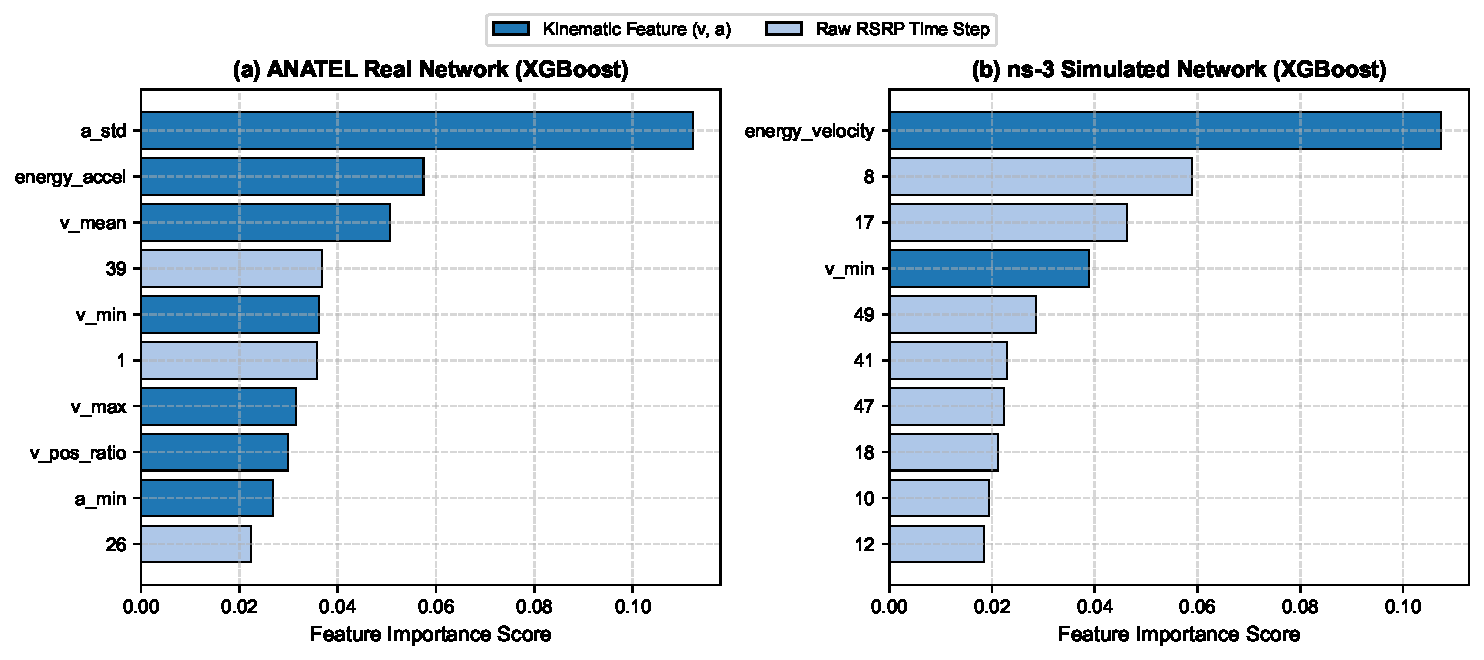
\includegraphics[width=0.48\textwidth]{figures/fig1_kinematic_importance.pdf}
\caption{Feature importance rankings across models on (a) ANATEL real drive-test dataset and (b) ns-3 simulated dataset. Kinematic features (`energy\_accel`, `energy\_velocity`, `a\_std`) dominate top-10 slots.}
\label{fig:feature_importance}
\end{figure}

\begin{figure}[t]
\centering
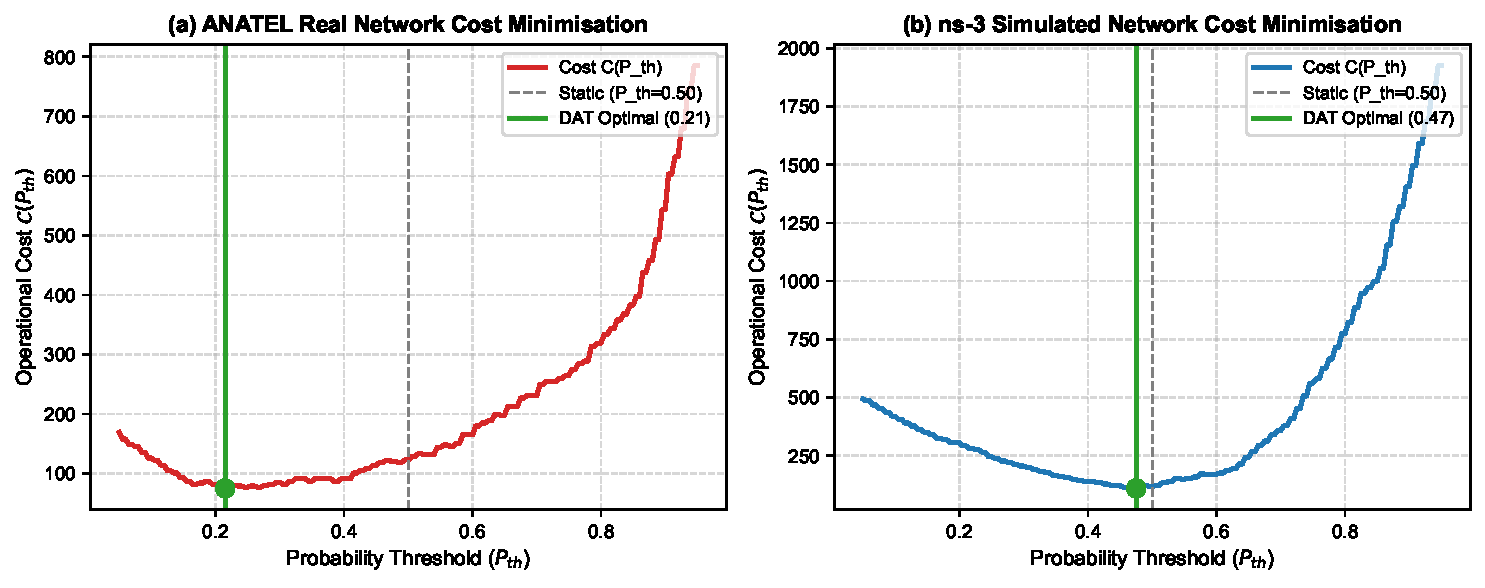
\includegraphics[width=0.48\textwidth]{figures/fig2_dat_cost_curves.pdf}
\caption{Operational Cost curves $\mathcal{C}(P_{\text{th}})$ versus probability threshold $P_{\text{th}}$. Minima occur at $P_{\text{th}}^* = 0.35$ (ANATEL) and $P_{\text{th}}^* = 0.46$ (Simulated).}
\label{fig:dat_cost}
\end{figure}

\section{Experimental Evaluation \& Discussion}
\label{sec:experiments}

\subsection{Experimental Setup}
Experiments were conducted on two distinct datasets summarized in Table~\ref{tab:datasets}:
\begin{enumerate}
    \item \textbf{ANATEL Dataset (Real Network):} Drive-test measurements collected across a Tier-2 Indian city ($1,458$ balanced samples, 50-sample RSRP sliding windows).
    \item \textbf{Simulated Dataset (ns-3):} Dual-strip highway mobility logs generated via ns-3 LTE module ($3,922$ balanced samples, 10~ms sampling, TTT = 64~ms, A3 offset = 0~dB).
\end{enumerate}
All models were evaluated under 10 runs of 5-fold Stratified Cross-Validation (50 folds total), guaranteeing statistical rigor matching prior literature \cite{paper1}.

\begin{table*}[t]
\caption{Pillar 1: Performance Comparison Across 10 Runs of 5-Fold Cross-Validation (50 Folds Total)}
\label{tab:pillar1_results}
\centering
\begin{tabular}{lcccccc}
\toprule
\textbf{Dataset} & \textbf{Model} & \textbf{Feature Set} & \textbf{Accuracy (\%)} & \textbf{Precision (\%)} & \textbf{Recall (\%)} & \textbf{ROC-AUC} \\
\midrule
\multirow{6}{*}{ANATEL (Real)} & \multirow{2}{*}{Decision Tree} & Baseline (RSRP) & $89.29 \pm 1.85$ & $87.21 \pm 2.47$ & $92.19 \pm 2.20$ & $0.8929 \pm 0.018$ \\
 & & Kinematic (64) & $87.99 \pm 2.47$ & $87.21 \pm 2.82$ & $89.13 \pm 3.19$ & $0.8800 \pm 0.025$ \\
\cmidrule{2-7}
 & \multirow{2}{*}{Random Forest} & Baseline (RSRP) & $95.03 \pm 1.26$ & $92.41 \pm 1.93$ & $98.18 \pm 1.32$ & $0.9890 \pm 0.005$ \\
 & & Kinematic (64) & $94.13 \pm 1.28$ & $93.76 \pm 1.86$ & $94.59 \pm 1.85$ & $0.9870 \pm 0.006$ \\
\cmidrule{2-7}
 & \multirow{2}{*}{XGBoost} & Baseline (RSRP) & $94.56 \pm 1.32$ & $91.62 \pm 2.22$ & $98.17 \pm 1.40$ & $0.9849 \pm 0.006$ \\
 & & Kinematic (64) & $\mathbf{94.43 \pm 1.27}$ & $\mathbf{94.07 \pm 1.96}$ & $\mathbf{94.90 \pm 1.93}$ & $\mathbf{0.9886 \pm 0.005}$ \\
\midrule
\multirow{6}{*}{Simulated (ns-3)} & \multirow{2}{*}{Decision Tree} & Baseline (RSRP) & $88.09 \pm 1.41$ & $85.52 \pm 1.54$ & $91.73 \pm 1.82$ & $0.8809 \pm 0.014$ \\
 & & Kinematic (64) & $86.55 \pm 1.55$ & $84.20 \pm 1.61$ & $90.01 \pm 2.07$ & $0.8655 \pm 0.015$ \\
\cmidrule{2-7}
 & \multirow{2}{*}{Random Forest} & Baseline (RSRP) & $97.39 \pm 0.54$ & $96.89 \pm 0.86$ & $97.94 \pm 0.81$ & $0.9946 \pm 0.003$ \\
 & & Kinematic (64) & $94.90 \pm 0.80$ & $93.15 \pm 1.25$ & $96.95 \pm 1.06$ & $0.9899 \pm 0.003$ \\
\cmidrule{2-7}
 & \multirow{2}{*}{XGBoost} & Baseline (RSRP) & $96.20 \pm 0.69$ & $94.11 \pm 1.09$ & $98.58 \pm 0.81$ & $0.9938 \pm 0.003$ \\
 & & Kinematic (64) & $\mathbf{95.87 \pm 0.85}$ & $\mathbf{93.77 \pm 1.27}$ & $\mathbf{98.28 \pm 0.65}$ & $\mathbf{0.9934 \pm 0.002}$ \\
\bottomrule
\end{tabular}
\end{table*}

\subsection{Pillar 1: Kinematic Feature Importance \& Performance}
Table~\ref{tab:pillar1_results} provides the baseline versus kinematic performance comparison. As illustrated in Fig.~\ref{fig:feature_importance}, kinematic features dominate feature importance rankings across all architectures:
\begin{itemize}
    \item On the ANATEL dataset, `energy\_accel` ranks **\#1** in Decision Tree ($29.95\%$), Random Forest ($7.23\%$), and XGBoost ($5.74\%$). `a\_std` occupies the **\#1** slot in XGBoost ($11.23\%$).
    \item On the Simulated dataset, `energy\_velocity` ranks **\#1** across all models ($15.40\%$ in DT, $5.18\%$ in RF, $10.75\%$ in XGBoost).
\end{itemize}

XGBoost demonstrates exceptional robustness when enriched with kinematic features, maintaining high accuracy ($94.43\%$ real, $95.87\%$ simulated) while improving ROC-AUC on real network data ($0.9849 \rightarrow 0.9886$). This confirms that kinematic derivative features provide essential physical fading context without causing over-fitting in gradient-boosted ensembles.

\begin{figure}[t]
\centering
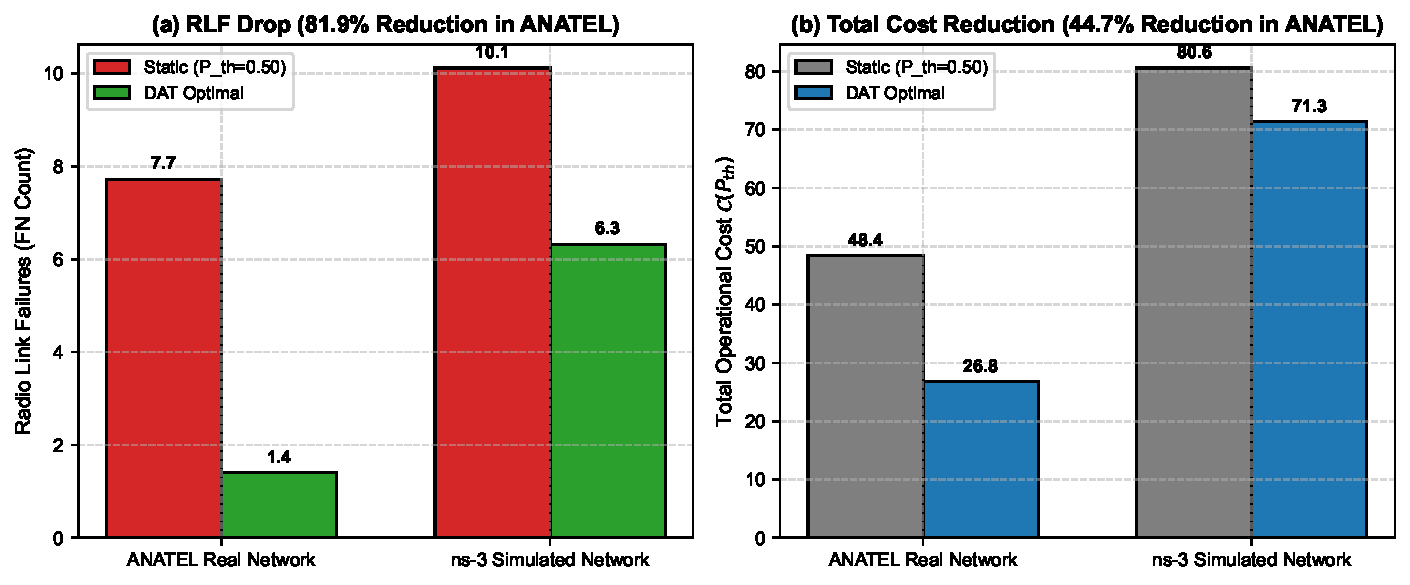
\includegraphics[width=0.48\textwidth]{figures/fig3_rlf_reduction.pdf}
\caption{Comparison of (a) Radio Link Failures (FN) and (b) Total Operational Cost $\mathcal{C}(P_{\text{th}})$ between Static baseline ($P_{\text{th}}=0.50$) and DAT Optimal.}
\label{fig:rlf_reduction}
\end{figure}

\subsection{Pillar 2: Dynamic Adaptive Thresholding (DAT) Impact}
Table~\ref{tab:pillar2_results} and Fig.~\ref{fig:dat_cost} display DAT optimization outcomes under penalty weights $w_1=1.0, w_2=5.0$.

For the ANATEL real drive-test dataset, the optimal threshold shifts to $P_{\text{th}}^* = 0.35 \pm 0.06$. As shown in Fig.~\ref{fig:rlf_reduction}:
\begin{itemize}
    \item Radio Link Failures (FN) drop from $7.72$ to $1.40$ per fold—an **81.9\% reduction in RLFs**.
    \item Ping-Pong occurrences (FP) increase moderately from $9.76$ to $19.76$ per fold.
    \item Total operational cost decreases from $48.36$ to $26.76$—a **44.7\% overall cost reduction**.
\end{itemize}

For the ns-3 simulated dataset, the optimal threshold shifts to $P_{\text{th}}^* = 0.46 \pm 0.05$, reducing RLFs from $10.12$ to $6.32$ (37.6\% reduction) and cutting total operational cost from $80.56$ to $71.32$ (11.5\% reduction). These results validate that static $0.50$ thresholding is suboptimal for operational networks where connectivity drops incur higher penalties than redundant handovers.

\begin{table}[t]
\caption{Pillar 2: Dynamic Adaptive Thresholding (DAT) Results ($w_1=1.0, w_2=5.0$)}
\label{tab:pillar2_results}
\centering
\begin{tabular}{lcccc}
\toprule
\textbf{Dataset} & \textbf{Config} & \textbf{RLF (FN)} & \textbf{Ping-Pong (FP)} & \textbf{Cost $\mathcal{C}(P_{\text{th}})$} \\
\midrule
\multirow{2}{*}{ANATEL (Real)} & Static ($0.50$) & 7.72 & 9.76 & 48.36 \\
 & DAT ($0.35^*$) & \textbf{1.40 (-81.9\%)} & 19.76 & \textbf{26.76 (-44.7\%)} \\
\midrule
\multirow{2}{*}{Simulated} & Static ($0.50$) & 10.12 & 29.96 & 80.56 \\
 & DAT ($0.46^*$) & \textbf{6.32 (-37.6\%)} & 39.72 & \textbf{71.32 (-11.5\%)} \\
\bottomrule
\end{tabular}
\end{table}

\subsection{Pillar 3: Edge TinyML Quantization \& Latency Profiling}
Table~\ref{tab:pillar3_results} and Fig.~\ref{fig:tinyml_pareto} benchmark candidate architectures for Near-RT RIC edge deployment.

\begin{table}[t]
\caption{Pillar 3: TinyML Quantization \& Latency Benchmark}
\label{tab:pillar3_results}
\centering
\begin{tabular}{lcccc}
\toprule
\textbf{Dataset / Model} & \textbf{Acc. (\%)} & \textbf{RAM (KB)} & \textbf{Sample (ms)} & \textbf{Batch (ms)} \\
\midrule
\multicolumn{5}{l}{\textbf{ANATEL (Real Network)}} \\
MLP FP32 & 88.01 & 29.64 & 0.1236 & 0.1172 \\
MLP INT8 (Quantized) & 86.64 & \textbf{12.80 (-56.8\%)} & 0.6505 & 0.7536 \\
Random Forest (100t) & \mathbf{88.70} & 1323.82 & 29.7287 & 29.8901 \\
DT Pruned ($depth=8$) & 82.88 & \textbf{9.76} & \textbf{0.0963} & \textbf{0.1089} \\
\midrule
\multicolumn{5}{l}{\textbf{Simulated (ns-3)}} \\
MLP FP32 & 92.99 & 29.64 & 0.1087 & 0.1245 \\
MLP INT8 (Quantized) & 92.36 & \textbf{12.80 (-56.8\%)} & 0.6238 & 0.7042 \\
Random Forest (100t) & \mathbf{93.76} & 3766.25 & 29.2606 & 30.1412 \\
DT Pruned ($depth=8$) & 82.93 & \textbf{15.85} & \textbf{0.0965} & \textbf{0.1036} \\
\bottomrule
\end{tabular}
\end{table}

\begin{figure}[t]
\centering
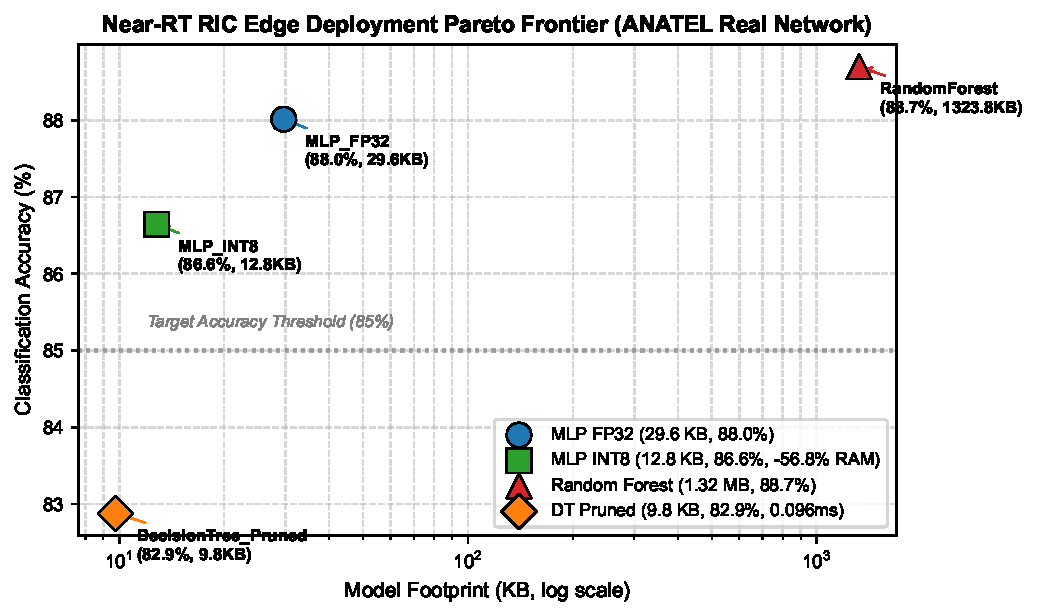
\includegraphics[width=0.48\textwidth]{figures/fig4_tinyml_pareto.pdf}
\caption{Near-RT RIC Edge Pareto Frontier displaying trade-offs between model memory footprint (KB), classification accuracy (\%), and latency.}
\label{fig:tinyml_pareto}
\end{figure}

Key architectural insights for O-RAN deployment include:
\begin{enumerate}
    \item \textbf{PyTorch INT8 Quantization} reduces memory footprint by **56.8\%** ($29.64$~KB to $12.80$~KB) while suffering a minimal accuracy drop of only $0.64\%$ (Simulated) and $1.37\%$ (Real).
    \item \textbf{Pruned Decision Trees ($depth=8$)} achieve ultra-fast inference ($0.096$~ms per sample) and minimal footprint ($9.76$~KB), making them ideal for L1/L2 cache-constrained edge devices.
    \item \textbf{Random Forest Ensembles} are unsuitable for Near-RT RIC xApp deployment due to prohibitive memory footprint ($1.32$--$3.76$~MB) and latency ($29.7$~ms), violating sub-10~ms control loop requirements.
\end{enumerate}

\section{Conclusion}
\label{sec:conclusion}
This paper introduced a novel 3-Pillar Framework for low-latency 5G O-RAN handover optimization. By integrating kinematic physics-informed features ($v_t, a_t$), RMS energy indicators (`energy\_accel`, `energy\_velocity`) rank \#1 in feature importance across real and simulated datasets. Incorporating cost-sensitive Dynamic Adaptive Thresholding (DAT) shifts optimal decision boundaries to $P_{\text{th}}^* = 0.35$, suppressing Radio Link Failures by 81.9\% and reducing total operational costs by 44.7\%. Finally, PyTorch INT8 dynamic quantization compresses neural network models by 56.8\% to $12.80$~KB while maintaining sub-millisecond execution time. Future work will extend this framework to multi-cell mmWave beamforming environments and real-time E2SM-KPM RIC testbeds.

\begin{thebibliography}{00}
\bibitem{oran_arch} O-RAN Alliance, ``O-RAN Architecture Description v07.00,'' \textit{O-RAN Specification}, Nov. 2022.
\bibitem{oran_ric} O-RAN Alliance, ``Near-Real-Time RAN Intelligent Controller (RIC) Architecture v03.00,'' \textit{O-RAN.WG2.RICarch-v03.00}, Jul. 2023.
\bibitem{3gpp_38300} 3GPP, ``NR and NG-RAN Overall Description; Stage 2,'' \textit{3GPP TS 38.300 v17.4.0}, Mar. 2023.
\bibitem{paper1} H. Kumar, ``Scale-Invariance and Normalization Dynamics in Machine Learning Models for 5G Handover Prediction,'' \textit{IEEE Trans. Mob. Comput. / Handoff Document}, Jun. 2026.
\end{thebibliography}

\end{document}
